\documentclass[conference, dvipdfmx]{IEEEtran} % 在後面加dvipdfmx才能新增pdf圖片
\IEEEoverridecommandlockouts
% The preceding line is only needed to identify funding in the first footnote. If that is unneeded, please comment it out.
\usepackage{cite}
\usepackage{amsmath,amssymb,amsfonts}
\usepackage{algorithmic}
\usepackage{graphicx}
% \usepackage[dvips]{graphicx}
% \usepackage[dvipdfmx]{graphicx}
\usepackage{textcomp}
\usepackage{xcolor}
\usepackage{float}
% package for code
% \usepackage{caption}

% table
% for Talbe centering with fixed width
\usepackage{array}
\usepackage{threeparttable}

%程式碼
\usepackage{varwidth}

\def\BibTeX{{\rm B\kern-.05em{\sc i\kern-.025em b}\kern-.08em
    T\kern-.1667em\lower.7ex\hbox{E}\kern-.125emX}}
\begin{document}
\begin{sloppypar}

\title{An Access Control System for Verifiable Credentials with Selective Disclosure\\
{\footnotesize \textsuperscript{*}Note: Sub-titles are not captured in Xplore and
should not be used}
\thanks{Identify applicable funding agency here. If none, delete this.}
}

\author{\IEEEauthorblockN{1\textsuperscript{st} Chun-An Lin}
\IEEEauthorblockA{\textit{Graduate school of Natural} \\ \textit{Science \& Technology}  \\
\textit{Kanazawa University}\\
Kanazawa, Japan \\
kimlin20011@gmail.com}
\and
\IEEEauthorblockN{2\textsuperscript{nd} Chen-Mou Cheng}
\IEEEauthorblockA{\textit{Graduate school of Natural} \\ \textit{Science \& Technology}  \\
\textit{Kanazawa University}\\
Kanazawa, Japan \\
cheng@se.kanazawa-u.ac.jp}
\and
\IEEEauthorblockN{3\textsuperscript{rd} Masahiro Mambo}
\IEEEauthorblockA{\textit{Graduate school of Natural} \\ \textit{Science \& Technology}  \\
\textit{Kanazawa University}\\
Kanazawa, Japan \\
mambo@ec.t.kanazawa-u.ac.jp}
% \and
% \IEEEauthorblockN{4\textsuperscript{th} Given Name Surname}
% \IEEEauthorblockA{\textit{dept. name of organization (of Aff.)} \\
% \textit{name of organization (of Aff.)}\\
% City, Country \\
% email address or ORCID}
% \and
% \IEEEauthorblockN{5\textsuperscript{th} Given Name Surname}
% \IEEEauthorblockA{\textit{dept. name of organization (of Aff.)} \\
% \textit{name of organization (of Aff.)}\\
% City, Country \\
% email address or ORCID}
% \and
% \IEEEauthorblockN{6\textsuperscript{th} Given Name Surname}
% \IEEEauthorblockA{\textit{dept. name of organization (of Aff.)} \\
% \textit{name of organization (of Aff.)}\\
% City, Country \\
% email address or ORCID}
}

\maketitle

\begin{abstract}
    It is important for access control mechanisms to consider both authentication and authorization components to enhance privacy and security. User-Managed Access (UMA) is an access control profile supporting (1) party-to-party sharing that allows the resource owner to authorize the resource to the third-party and (2) customization of access control policy which means resource owner can formulate the policy for accessing the protected resource. However, although the UMA profile defines the authorization process, it does not specify the detail part for authentication. To fill this gap, it is necessary to import digital credential technology to authenticate the third party. Therefore, this paper proposes VC-UMA, an access control mechanism integrating UMA with Verifiable Credentials (VC). VC is an open standard of decentralized credentials which often constructed on the blockchain that allowing user to fully control their credentials.  Besides, selective disclosure mechanism is integrated into VC-UMA to address the privacy concerns raised by sharing VCs. To prove the feasibility of the VC-UMA, the proof of concept is conducted. Specifically, a prototype system is implemented and the experiments of the performance is presented. 
\end{abstract}

\begin{IEEEkeywords}
    User-Managed Access, Verifiable Credentials, Access Control, Selective Disclosure, Blockchain
\end{IEEEkeywords}

\section{Introduction}

Access Control\cite{AccessControl1} is a mechanism responsible for managing the requests that want to access protected resources. Without proper access control mechanisms, internet services are prone to various privacy and security issues. For instance, invalid access to protected resources, or leakage of privacy data during the access control process.

User-Managed Access (UMA)\cite{UMA} is a party-to-party right delegation profile extension for access control. In UMA, users can not only formulate the customized access control policy\cite{UMA_paper1} but also realize the \textit{Party-to-Party Sharing} scenario. Nevertheless, according to Sandhu\cite{AccessControl_principle}, secure access control requires several important components namely, \textit{Authorization}, \textit{Authentication},  \textit{Auditing}, etc. Especially, authorization and authentication play extremely important roles in the process of user access to the protected resources.
However, UMA profile only defines the claim gathering concept for the authentication part which means the user needs to provide the claim to get authentication, but the trust model among all the entities is out of scope. For example, as a resource owner, the problem of \textit{how can I trust the third party to access the resources?} cannot be solved only by employing the UMA profile. 


To solve the above problems, this paper adopts Self-Sovereign Identity (SSI), a promising concept that is regarded as the next generation of digital identity\cite{Path_to_Self_Sovereign}. This concept allows individuals fully control of their digital identities and credential. Among SSI, Verifiable Credential (VC)\cite{VC_model} is a  core technology that is the digital credential framework of following the SSI principle and specifies by the World Wide Web Consortium (W3C). VC utilizes digital signature technology often together with the blockchain which is a distributed ledger platform with decentralized, immutable, and traceable features. With the wide acceptance of VC, privacy has become an important issue. Regarding the privacy issue, W3C recommends developers follow the data minimization principle\cite{VC_Implementation_Guidelines} when designing VC services. This means that when presenting VCs, is it better to minimize the exposed data to prevent oversharing of the privacy credentials. 
% \subsection{Research Objective}

Based on the above observations, this paper aims to propose a Verifiable Credential-enabled User-Managed Access Mechanism 
(VC-UMA) that overcomes the lack of trust authentication model defined in the UMA profile by introducing the advantages of the VC framework. Additionally, in order to reduce the risk of private data leakage when sharing VCs, this paper adopts the selective disclosure technology so that VC holder can redact the private part of data in VC to follow the data minimization principle.
To summarize, this paper claims the following contribution.

\begin{itemize}
  \item \textbf{An access control mechanism based on decentralized credential scheme is presented.}	This paper proposes a new access control mechanism: VC-UMA based on the W3C's VC model\cite{VC_model} and the UMA Profile\cite{UMA}. Besides, the relationship and the trusted model among all entities in UMA and VC is reconsidered. Moreover, the guidelines for implementing VC-UMA are provided in static and dynamic ways.
  \item \textbf{Selective disclosure method to achieve the data minimization principle for VC sharing is considered.} Considering the part of privacy-preserving VC sharing, we adopt the selective disclosure methods provided by W3C, a selective disclosure authentication flows is proposed.
  \item \textbf{A use case of VC-UMA has been proposed and implemented as the prototype system as proof of concept.}
  In order to prove the feasibility and usability of the proposed mechanism, the proof of concept research method is conducted. The implemented prototype system is presented. Furthermore, the performance of the system is analyzed.
\end{itemize}

% The rest of the paper is organized as follows. In Section \ref{sec:back}, the background and related work is organized; The proposed VC-UMA mechanism is discussed in Section \ref{sec:system_design}; Then, Implementation and experiments of prototype system based on the provided use case is presented in Section \ref{sec:Evaluation}. In Section \ref{sec:Conclusion}, the conclusion of this paper is summed up.

\section{Background and Related Work}
\label{sec:back}
\subsection{User-Managed Access}


UMA is an access control profile base on OAuth2\cite{OAuth2}, proposed by Kantara Initiative and published on Internet Engineering Task Force (IETF) \cite{UMA}. 
OAuth2 is a  widely used third-party authorization protocol, but this protocol doesn't cover the party-to-party sharing scenarios.
For instance, Alice wants to use the service of photo editing software (playing the role of resource access client), so she authorizes her photos (resource) stored in the third-party cloud service to the photo editing software. However, OAuth2 doesn't support Alice to grant Bob to access her photos on the third-party cloud service.
UMA fills the gap of OAuth2 that doesn't define the party-to-party authorization scenario. 
UMA profile is composed of several entities, the definitions of which are shown in table \ref{table:UMA_entities}.

% According to the UMA Profile\cite{UMA}, the UMA process can be divided into three phases, namely \textit{Protecting a Resource}, \textit{Getting Authorization} and \textit{Accessing a Resource}. First, in the \textit{Protecting a Resource} phase, RO registers RS to AS. After registration, RS will obtain the Protection API Token (PAT) from the AS. After that, RO then registers the access policy of the protected resource to AS; the \textit{Getting Authorization} phase mainly refers to RqP requesting authorization from AS through Client. In this process, RqP is required to present the claims related to the access policy in order to get authenticate from AS. After passing the verification, Client will obtain the Requesting Party Token (RPT) from AS; Finally, in \textit{Accessing a Resource} phase, Client may reaccess the protected resource by sending the access request accompanied by the RPT to RS.

\begin{table}[htbp]
  \caption{Entities in User-Managed Access}
  \label{table:UMA_entities}
  \small
  \scalebox{0.9}{
  \begin{tabular}{>{\centering\arraybackslash}p{2.2cm} p{6cm}l}
  \hline
  UMA entities	& description \\ \hline\hline
  Resource Owner (RO)	& The owner of the protected resource.\\ \hline
  Requesting Party (RqP)	& The party who is attempting to access the protected resource.\\ \hline
  Client	& A third-party application that proxy the RqP to access protected resources.\\ \hline
  Resource Server (RS)	& The resource server stores protected resources and is capable of handling resource requests from client.\\ \hline
  Authorization Server (AS)		& The Authorization server is delegated by the RO to protect resources stored in RS and authorizes resource requests issued by RqP.\\ \hline
  \end{tabular}
  }
\end{table}


\subsection{Blockchain and Smart Contract}
Blockchain is regarded as the core technology underlying Bitcoin\cite{bitcoin}. The underlying technology of blockchain is distributed ledgers, which is regarded as a decentralized platform with immutability, transparency, and traceability. Recently, some blockchain platforms also brought out a new idea called Smart Contract\cite{blockchain_smart_contract}, which allows developers to run program logic that can be used to verify and execute transactions. Ethereum\cite{ethereum} is a famous blockchain platform that not only allows user to compile and deploy smart contracts but also change the account status or interact with other accounts. Furthermore, Ethereum provides Ethereum Virtual Machine (EVM) to compile and run Turing-complete smart contract languages (e.g., Solidity, Vyper, etc.) Therefore, developers can run decentralized applications (DApp) in the blockchain in the form of smart contracts. Compared with Bitcoin, Ethereum is more scalable and flexible for the development of software applications on blockchain.

\subsection{Decentralized Identifiers and Verifiable Credentials}

Decentralized identifiers (DID) is one of the important technologies of SSI. DID is a digital Identity framework build over decentralize infrastructure such as blockchain. In DID framework, user doesn't need to rely on the centralized identity service to create a personal digital identity. The composition of the DID is usually composed of a series of random numbers, for example, $DID:example:0x2e12sfhx...$. This shows that DID is a high degree of anonymity. On the other hand, since a user can possess multiple DID at the same time, user activities can be prevented from being correlated which leads to the improvement of privacy. Besides, In the DID scheme, each DID will be connected to a corresponding DID Document, which mainly contains the public verification keys and related verification data. Specifically, since the storage location of the DID and DID Document is usually recorded in Blockchain, the DID owner can easily use the public key in the DID Document to claim ownership.

In many identity verification scenarios, \textit{Verifiable Properties} are required. For instance, Alice needs to prove that she is graduated from university.  To fill this gap, SSI also provides an important technology called \textit{Verifiable Credentials} (VC). VC includes three important roles shown in Figure \ref{fig:vc_framework}. \textit{Holder} is the entity that owns and controls VC; \textit{Issuer} is a trusted third party responsible for VC issuance; \textit{Verifier} is the entity that wants to verify the VC. VC Framework is built on top of the Verifiable Data Registry (VDR) and DID technology. VDR is generally implemented by blockchain in order to take benefit of blockchain decentralized features. Take the school issuing graduation certificate as an example. First, both the student (Holder) and the school (Issuer) need to register their unique DIDs to VDR in advance. After that, Issuer packs and signs the student's DID, claims, and related certificate information by DID to generate VC. After obtaining VC, Verifier can find the DID Document through the issuer's DID in the VDR to obtain the public key and then verify the signature in the VC.


\begin{figure}[ht] %浮動式圖形htbp
  % \begin{center} %中央寄せ
  \centering  
  % 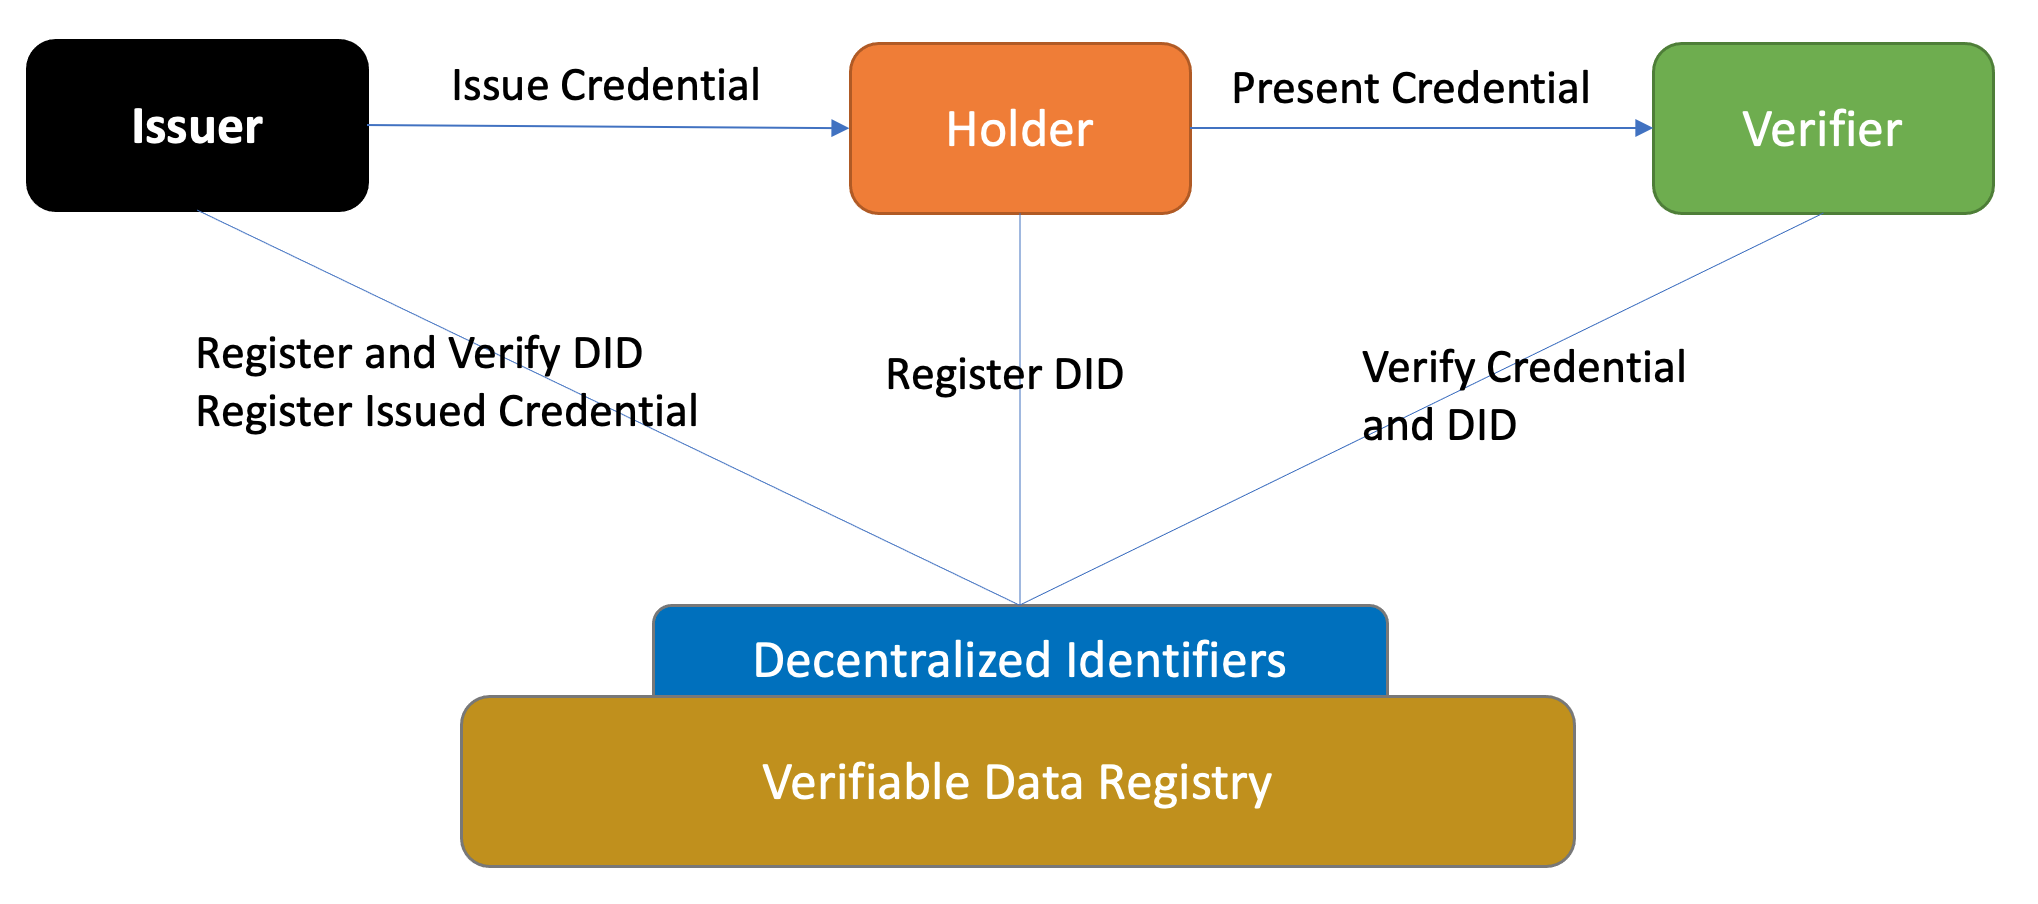
\includegraphics[width=83mm]{images/vc_framework.png} %[サイズ]{ファイル名.png}
  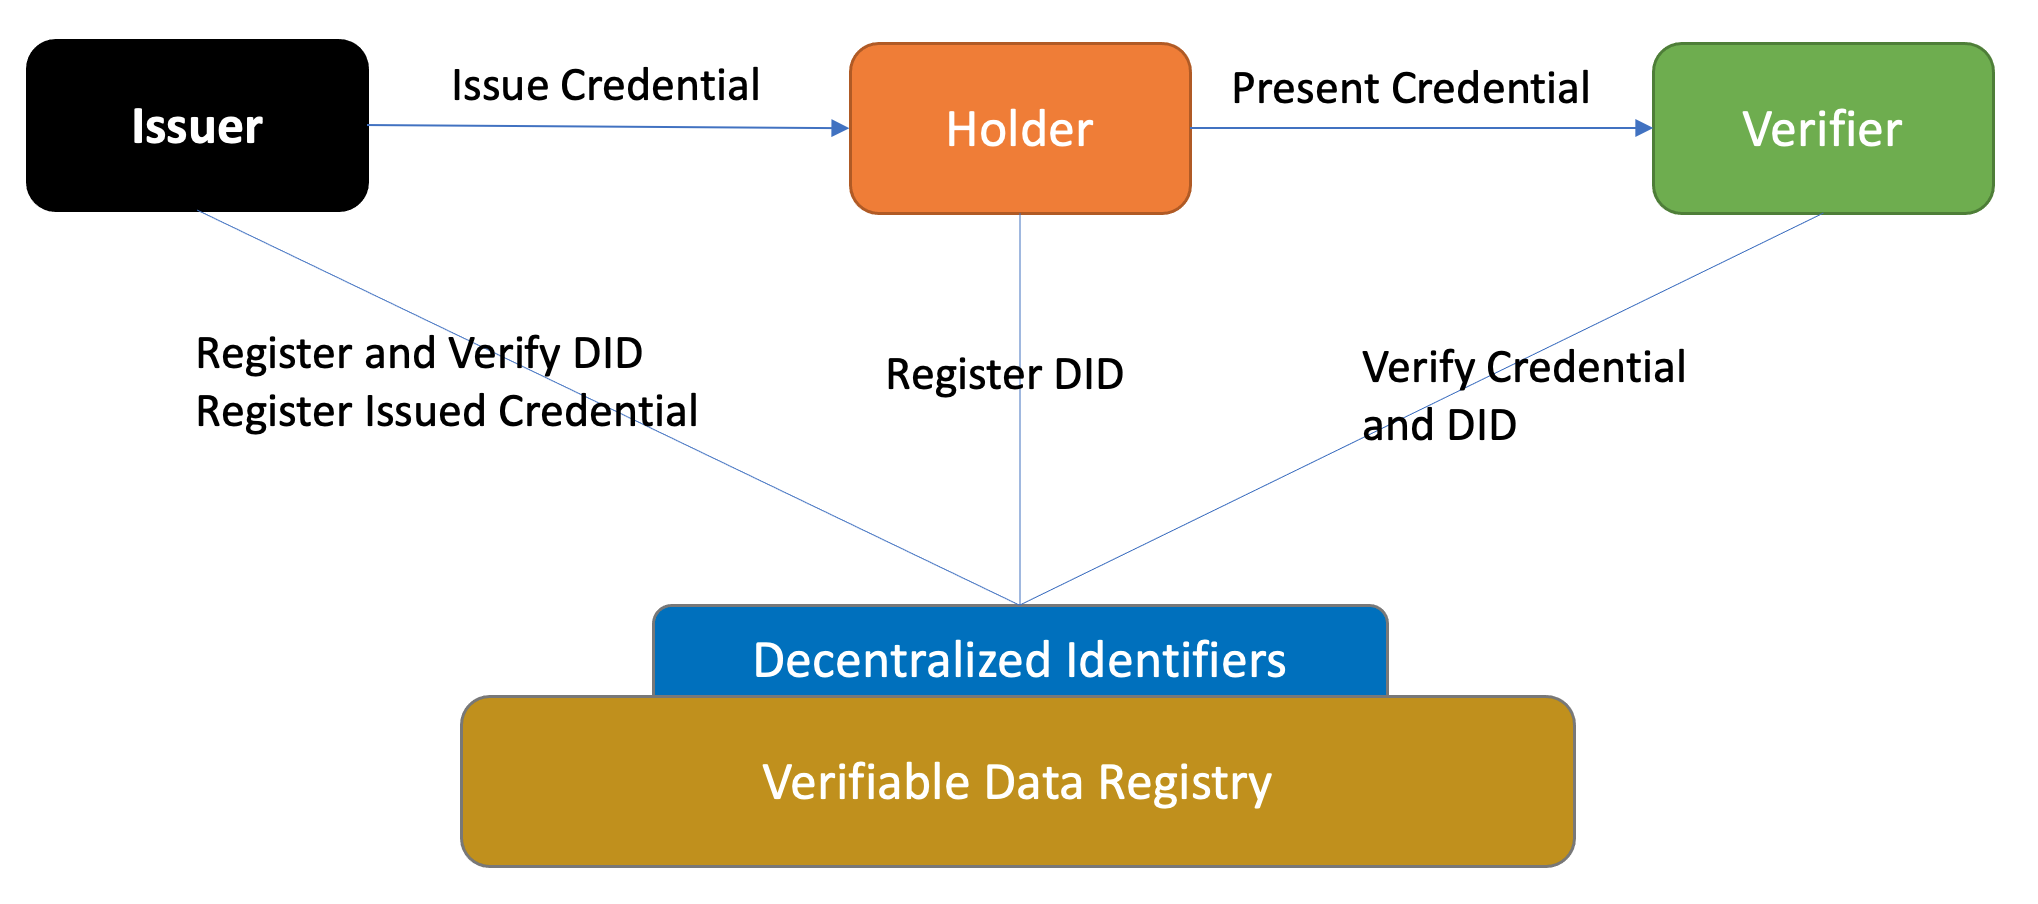
\includegraphics[width=83mm]{images/vc_framework.png} %[サイズ]{ファイル名.png}
  \caption{The roles and information flows for Verifiable Credential} %キャプション
  \label{fig:vc_framework} %ラベル名label
  % \end{center}
\end{figure}


As the VC technology is still in the development stage, there are still many problems to be solved. One of the potential problems is privacy violations.  For preventing privacy violations, the generally accepted best practice is data minimization. In order to achieve the data minimization principle, Selective disclosure techniques is recommended to be used in the issue or present stage of VC\cite{VC_model}.  {Selective disclosure signatures} are commonly realized by the zero-knowledge proof cryptography method in order to allow the VC holder to hide the private attributes in VC. There are some developing signature schemes that can be natively applied to selective disclosure signatures systems, such as Camenisch-Lysyanskaya (CL) signature\cite{cl_sig} and BBS+ signature\cite{bbs_1}. Compared with CL Signature, BBS+ signature can achieve considerable security through much shorter keys and signatures\cite{bbs_cl}. Therefore, this paper not only adopts BBS+ signature technology to support the signature scheme for VC but also apply to the zero-knowledge proof for selective disclosure signatures method. 

\subsection{Related Work}
In recent years, there are many studies dedicated to utilizing SSI technology to improve privacy and security for access control mechanism. CredChain\cite{Selective_Disclosure_paper} provides an SSI platform that enables issuer and VC holder to create, share and verify credentials in a safe environment. In consideration of personal privacy issues, this paper also leverages redactable signature\cite{redactable_signature} method allowing users to hide the secret attribute in credential; CanDID\cite{CanDID} is a user-friendly decentralized identity platform that is committed to achieving Sybil-resistance, accountability, key recovery, and other goals in a privacy-preserving way; Lagutin et al.\cite{VC_Oauth} proposed a DID and VC enabled OAuth-based delegation network. They attempt to establish an OAuth-based access control framework through the introduction of DID and VC technology to solve the problem of OAuth2 which does not cover the authentication profile.  However, this study only made a preliminary process design for the framework but didn't consider the privacy issue of VC as well as the party-to-party sharing issue often encountered in IoT scenarios.

To overcome the issues mention in advance, this paper is committed to designing a \textit{privacy-preserving access control mechanism} that focuses on both \textit{Authorization} and \textit{Authentication} domain in the access control mechanism. Besides, the proposed mechanism is based on the UMA profile to support the party-to-party sharing scenario. Moreover, by introducing promising DID and VC technologies, the proposed mechanism allows users to participate in the access control process while also protecting the privacy of the personal credentials presented by themselves.

\section{System Design}
\label{sec:system_design}

In order to overcome the aforementioned issues, this paper is dedicated to designing a \textit{Privacy-Preserving Verifiable Credential-enabled User-Managed Access} Mechanism, and named it VC-UMA. VC-UMA is a user-centralize access control mechanism, which contains two subdomains, namely VC domain and UMA domain. UMA domain refers to UMA Profile\cite{UMA}; The VC domain refers to the decentralized identity technology in SSI, such as DID and VC. Besides, the notation used in this paper are listed in Table \ref{table:notation}. 
While designing the overall system, we also commit to achieving the following goals.

\begin{table}[ht]
  \begin{center}
  \caption{Notation}
  \label{table:notation}
  % \begin{tabular}{c|p{28em}l}
    \scalebox{0.9}{
      \begin{tabular}{c p{6cm}l}
      \hline
      Notation	& Description \\ \hline\hline
      $doc$	& DID Document\\ \hline
      $pk$	& Public key\\ \hline
      $sk$	& Secret key\\ \hline
      $\sigma$	& Signature by $sk$ over $id$ and subject\\ \hline
      $\pi$	& Proof\\ \hline
      $CS$	& The set of claims\\ \hline
      $ctx$	& Context\\ \hline
      \end{tabular}
    }
  \end{center}
\end{table}


\begin{enumerate}
  \item \textbf{Decentralization of credential issuance system: trusted and high availability.} The centralized credential issuance system has disadvantages such as the risk of signal point of failure. Therefore, importing a decentralized credential issuance scheme is the primary goal of this paper.
  \item \textbf{Privacy of Credential.} When utilizing VC technology, privacy data leakage of the credential is also an important issue. Hence, the introduction of the related technology of privacy-preserving VC is also one of the goals of this paper.
  \item \textbf{Compact Size of Privacy-Preserving Cryptographic.} Privacy-preserving VC technology often requires the usage of encryption methods, such as zero-knowledge Proof. However, related technologies often require considerable computer resource(e.g., zk-SNARKs). Therefore, this paper is committed to employing the privacy-preserving cryptographic that can achieve the high-level security which only requires compact size of computing and storage resources.
\end{enumerate}

\subsection{System Architecture}

As shown in Figure \ref{fig:system_architecture}, the access control mechanism is divided into the UMA domain and VC domain. Among them, the UMA domain is responsible for handling the authorization management of protected resources and the verification of the requesting party (RqP);
The VC domain defines the process for RqP to obtain VC. Besides, we assume that RO, RS, and RqP already own DID which corresponds to the private key, public key, and DID Document registered to the Verifiable Data Registry (VDR). In addition, anyone can directly obtain the DID Document corresponding to the DID through VDR.


\begin{figure}[htbp] %浮動式圖形
  \begin{center} %中央寄せ
  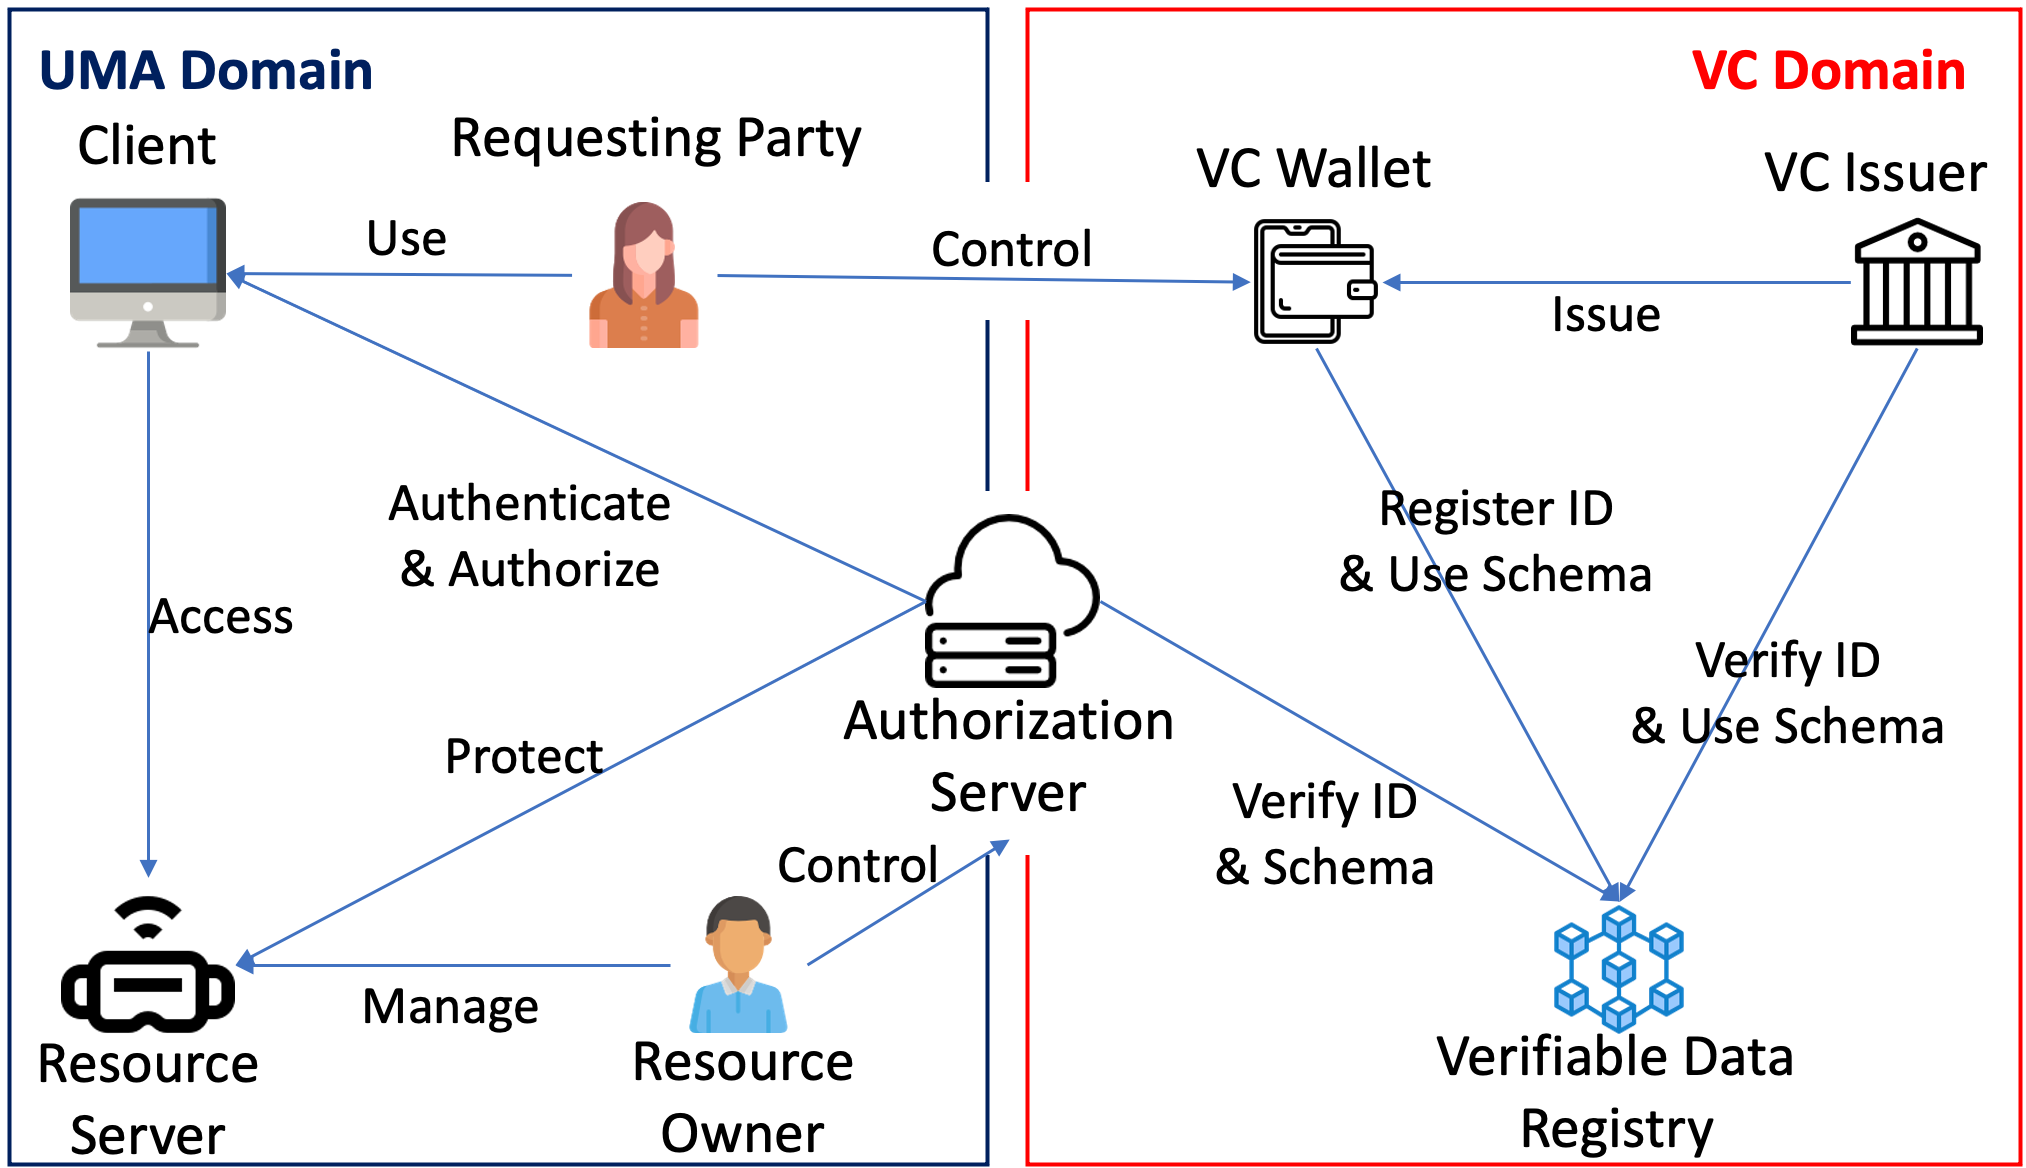
\includegraphics[width=0.47\textwidth]{images/structure_vc_uma.png} %[サイズ]{ファイル名.png}
  \caption{System Architecture of VC-UMA} %キャプション
  \label{fig:system_architecture} %ラベル名label
  \end{center}
\end{figure}

The UMA Domain mainly refers to the entities defined in UMA Profile\cite{UMA}.
RO is the provider of protected resources, responsible for the management of RS, and defines the access control policy of RS through AS;
RqP is a third party that wants to access protected resources; 

In VC Domain, there are four roles (1)\textbf{VC issuer} is responsible for issuing and releasing VC to RqP; (2)\textbf{VC wallet} owned by RqP which supports storing and managing VC as well as DID; (3)\textbf{Verifiable Data Registry (VDR)} is a decentralized infrastructure such as blockchain that supports the registration and resolution for DID, DID Document, and VC status; (4)\textbf{Authorization Server (AS)}  represents the role of VC verifier in the VC model. Besides, AS also response for verifying whether the Verifiable Presentation (VP) provided by the VC wallet complies with the access control policy or not.

\subsection{Smart Contracts for VC domain}
The VDR of VC Domain needs to be maintained by SSI service provider (a trusted party that provides SSI implementation standards. It can be a third party or VC issuer) To set up the VC Domain process, SSI service provider needs to deploy \textit{VC Registry Contract} to VDR.

Considering the difference between \textit{Selective Disclosure Signatures} flow and \textit{Atomize Information} flow, this paper provides two kinds of \textit{VC Registry Contract} support these two flows as follows.
\begin{itemize}
  \item 	\textbf{Selective Disclosure Signatures Flow}\\
  Specifically, because the \textit{Selective Disclosure Signatures} flow hides the claims in the VC through encryption technology to ensure that sensitive information is not disclosed, the VC issuer does not need to modify the VC generation method provided by the W3C VC document.
  \item \textbf{Atomize Information Flow}\\
  In order to protect the privacy of claims in VC, VC issuer separates $n$ claims and then issue $n$ VCs, denoted as $\{VC_n\}$,  which one VC only include one claims. In this research, the set of $\{VC_n\}$ is defined as $VC\_Set$.
\end{itemize}

The design of VC Registry Contract for Selective Disclosure Signatures Flow refer to Figure \ref{fig:VC_Registry_API_sd_flow}.  It mainly includes \textit{register} and \textit{revoke} API for VC issuer to register and revoke VC, while \textit{isRevoked} API provides verifier to query the status whether a VC has been revoked or not;
The design of VC Registry Contract API for Atomize Information flow shown in Figure \ref{fig:VC_Registry_API_ai_flow}. After generating $VC\_Set$, VC issuer assigns a $VC\_Set\_id$ for $VC\_Set$, and then register $VC\_Set$ and $\{VC_n\}$ to the smart contract by invoking $register\_set$ and $register\_VC$ API respectively. 
Issuer can also revoke the $VC\_Set$ through the revoke API, and verifier can check the revocation status of the $VC\_Set$ by querying \textit{isRevoked} API.

\begin{figure}[htbp]
  \centering
  % \begin{center}
  % \begin{varwidth}{\dimexpr\textwidth-13\fboxsep-13\fboxrule\relax} % the width of fbox
  \begin{varwidth}{8.5cm}
  \fbox
  {\parbox{\textwidth}
    {
      \begin{center}
        \textbf{VC Registry Contract API (Selective Disclosure Signatures Flow)}
      \end{center}
      % - $register(vc\_id)$: The VC issuer registers the VC to the VC registry by issuer's blockchain account. \\ \\
      % - $revoke(vc\_id) 	\rightarrow true \lor false$: The VC issuer revokes the exist VC on the VC registry by issuer's blockchain account. \\ \\
      % - $isRevoked(vc\_id, issuer)  \rightarrow true \lor false$: The verifier can verify whether the VC have already been revoked or not. 
      \begin{itemize}
        \item $register(vc\_id)$: The VC issuer registers the VC.
        \item $revoke(vc\_id) 	\rightarrow true \lor false$: The VC issuer revokes the exist VC. 
        \item $isRevoked(vc\_id, issuer)  \rightarrow true \lor false$: The verifier can verify whether the VC have been revoked or not. 
      \end{itemize}
    }
  }
  \end{varwidth}
  % \end{center}
  \caption{VC Registry Smart Contract API}
  \label{fig:VC_Registry_API_sd_flow}
\end{figure}

\begin{figure}[H]
  \centering
  \begin{center}
  \begin{varwidth}{8.5cm}
  \fbox
  {\parbox{\textwidth}
    {
      \begin{center}
        \textbf{VC Registry Contract API (Atomize Information flow)}
      \end{center}
      \begin{itemize}
        \item $register\_set(vc\_set\_id, include\_type)$: The VC issuer registers the $vc\_set\_id$ and provides the $include\_type$ which represent the type of VCs included in VC set.
        \item $register\_VC(vc\_id, vc\_type, vc\_set\_id)$: The VC issuer registers the VC which include in the registered VC Set to the VC registry by issuer’s account.
        
        \item $revoke(vc\_set\_id)  	\rightarrow true \lor false$: The VC issuer revokes the existing VC set in the VC registry by issuer’s account.
        
        \item $isRevoked(vc\_set\_id)  \rightarrow true \lor false$: The Verifier can verify whether the VC set has already been revoked or not.
      \end{itemize}
    }
  }
  \end{varwidth}
  \end{center}
  \caption{VC Registry Smart Contract API (Atomize Information flow)}
  \label{fig:VC_Registry_API_ai_flow}
\end{figure}

\subsection{VC Domain Execution Flow}
In terms of the execution flow of VC-UMA. First, in the VC domain, VC issuer should issue VC following the Selective Disclosure Signatures flow or Atomize Information flow as follows.


\begin{itemize}
  \item \textbf{Selective Disclosure Signatures flow}\\
  \begin{enumerate}
    \item The VC issuer obtains the RqP's $DID_{RqP}$, and then verifies the $DID_{RqP}$ through VDR.
    \item 
    The VC issuer prepares $i$ claims to be issue, CS=$\{claim_i\}$, then signs the claims by $DID_{issuer}$ corresponding public and private key.	Denoted as $\sigma$ $\leftarrow$ $BBS\_PLUS$($DID_{RqP},$ $DID_{issuer},$ $(sk,pk)_{issuer},$ $CS)$ 
    \item Generate VC, denoted as $VC = \{metadata,CS, \sigma\}$
    \item VC issuer invokes the \textit{register} API of VC Registry to register the VC identifier.
    \item VC issuer send the VC to the VC wallet controlled by RqP.
  \end{enumerate}
  \item \textbf{Atomize Information Flow}
  \begin{enumerate}
    \item The VC issuer obtains the VC subject's (RqP) $DID_{holder}$, and then verifies the $DID_{holder}$ through VDR.
    \item \label{itm:sec}
    The VC issuer prepares $i$ claims to be issue, CS=$\{claim_i\}$, then signs the claims by $DID_{issuer}$ corresponding public and private key.	Denoted as \\$\sigma_i$ $\leftarrow$ $BBS\_PLUS$$(DID_{holder},$ $DID_{issuer},$ $(sk,pk)_{issuer},$ $claim_i)$
    \item \label{itm:thr} Generate VC. $VC_i = \{metadata, claim_i, \sigma_i\}$
    \item VC issuer repeats the step \ref{itm:sec} and \ref{itm:thr} $i$ times, then generates VC set, defined as  $VC\_SET = \{VC_i\}$. After that issuer assigns the $VC\_Set\_id$ as the identifier of $VC\_SET$
    \item VC issuer invokes the \textit{register} API of VC Registry to register the $VC\_Set\_id$.
    \item VC issuer send the $VC\_SET$ and $VC\_Set\_id$ to the VC wallet controlled by RqP.
  \end{enumerate}
\end{itemize}

\subsection{UMA Domain Execution Flow}

According to the UMA Profile\cite{UMA}, the VC-UMA mechanism process can be divided into three phases, namely \textit{Protecting a Resource}, \textit{Getting Authorization}, and \textit{Accessing a Resource}.

\subsubsection{Protecting a Resource Phase}

First, in the Protecting a Resources phase (Figure \ref{fig:ProtectResource}), RO needs to apply for registration for RS from AS.
At the same time, RO needs to provide resource DID, resource name, and PAT which prove that the registration is issued by the RO. 
After receiving the registration request sent by RS, AS verifies the existence of the resource DID and verifies the integrity of the DID Document through DID Registry. If the resource DID is verified, the AS will return a unique resource ID to the RS.

The second step is \textit{setPolicy}. At this step, RS must provide policySchema (JSON format), PAT (for authenticating RO), and resource ID (for identifying RS).
Among them, \textit{policySchema} provides the format for RqP to generate the Verifiable Presentation (VP) used in the Getting Authorization Phase; \textit{policySchema} represents the standard for verifying VP (e.g., age over 18).

\begin{figure}[htbp] %浮動式圖形
  \begin{center} %中央寄せ
  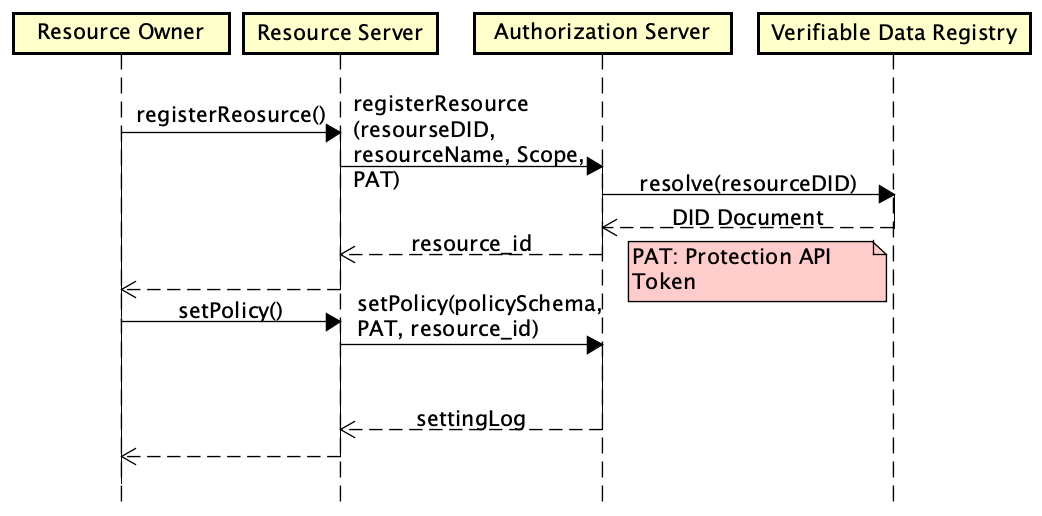
\includegraphics[width=83mm]{images/ProtectResource.png} %[サイズ]{ファイル名.png}
  \caption{Protecting a Resource Phase} %キャプション
  \label{fig:ProtectResource} %ラベル名label
  \end{center}
\end{figure}


\subsubsection{Getting Authorization Phase}
According to the UMA Profile, the Getting Authorization phase is divided into two steps. The first step is that RqP requests resource from RS through Client (Figure \ref{fig:GetAuthorization_Permission_Endpoint}). Since Client's request has not been authorized yet, so RS will directly apply for request permission from the Permission Endpoint of AS. After that, AS will return $permission Ticket$, $policySchema$, $as\_uri$ to Client.

\begin{figure}[htbp] %浮動式圖形
  \begin{center} %中央寄せ
  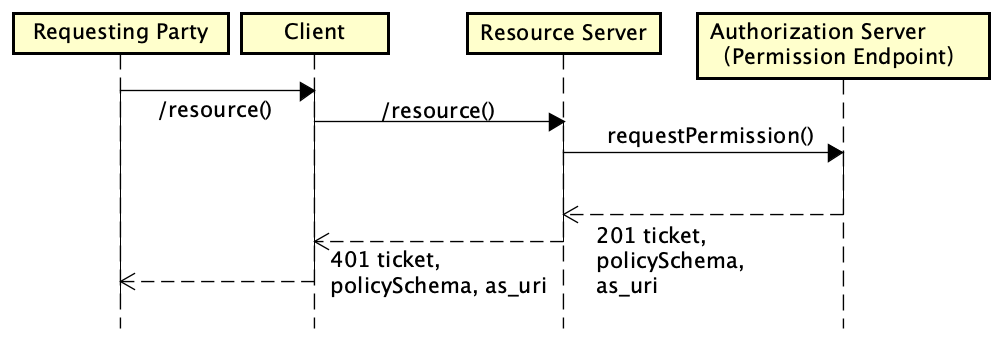
\includegraphics[width=83mm]{images/GetAuthorization_Permission_Endpoint.png} %[サイズ]{ファイル名.png}
  \caption{Getting Authorization Phase (Permission Endpoint)} %キャプション
  \label{fig:GetAuthorization_Permission_Endpoint} %ラベル名label
  \end{center}
\end{figure}

The second step of the \textit{Getting Authorization} phase is that the Client requests an RPT from the Token Endpoint in AS by providing a VP (Figure \ref{fig:GetAuthorization_Token_Endpoint}). This step is divided into two stages: \textit{Deriving Verifiable Presentation} and \textit{Releasing RPT}.

In the \textit{Deriving Verifiable Presentation} Stage, the Client alerts RqP that it requires using VC wallet for identity verification. Specifically, RqP can use VC wallet to obtain credential requests (in practice, it is common to use QR code). After accepting the credential request,  VC wallet can alert RqP of the claims that need to be presented according to \textit{policySchema} accompanied by the request.
Then, RqP can choose $k$ claims that it wants to share to the AS  among the VCs with $i$ claims, which can be expressed as $CS_k = \{claim_k\}$. 
After that, VC wallet derives proof from VC by \textit{BBS+ Signature Proof Generation} method. Derived proof can be expressed as $\pi = BBS+ ProofGen(pk_{issuer}, CS_{i-k}, CS_k, \sigma)$. Then VC wallet can use the derived proof to generate derived VC, expressed as $VC_{derived} = \{ctx, CS_k, \pi\}$. Finally, VC wallet package the derived VC into VP and send back to AS. VP can be expressed as $VP=\{ctx, VC_{derived}, \pi\}$.

\begin{figure}[htbp] %浮動式圖形
  \begin{center} %中央寄せ
  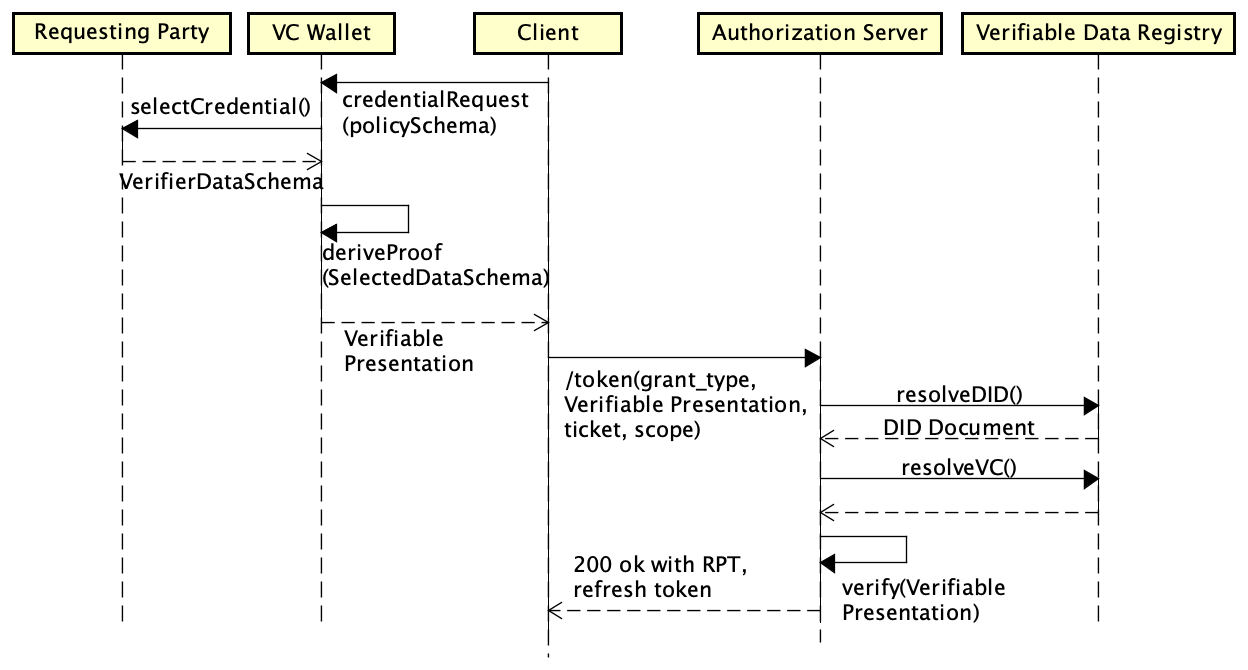
\includegraphics[width=83mm]{images/GetAuthorization_Token_Endpoint.png} %[サイズ]{ファイル名.png}
  \caption{Getting Authorization Phase (Token Endpoint)} %キャプション
  \label{fig:GetAuthorization_Token_Endpoint} %ラベル名label
  \end{center}
\end{figure}

At last, in the \textit{Releasing RPT} Stage, the AS first obtains the resource request information according to the \textit{ticket}. Then AS verifies the VP provided by VC wallet and confirms whether it meets the requirements of the policy or not. Furthermore, AS also needs to verify whether the DID of the VC issuer is legal through the VDR. When all verifications are passed, AS returns an RPT to the Client.

\subsubsection{Accessing a Resource Phase}
After successfully obtaining the RPT in the previous phase, the client first sends an RPT-accompanied request to the RS again. After that, the RS redirects the RPT to the AS's token introspect endpoint for verification. 
Then, AS returns the verification result (token introspection object) back to the RS. Finally, if the result is successful, RS can start to allow the client to access the protected resource.

\section{Evaluation}
\label{sec:Evaluation}

This section illustrates the feasibility of the VC-UMA by proof of concept. The prototype system is introduced. In addition, the experiments and the analyzation of prototype system is reported.

\subsection{Feasibility}

The prototype system is divided into \textit{VC Setup Side} and \textit{Access Control Side}. \textit{VC Setup Side} includes VC issuer, which mainly implements VC domain execution flow; \textit{Access Control Side} includes Alice's (requesting party) device, resources, and authorization server owned by Bob (Resource Owner), mainly implement the UMA domain execution flow. In order to communicate with smart contracts, VC issuer, authorization server, and Alice's device are required to deploy blockchain node.

The backend of the prototype system is developed in TypeScript language. Furthermore, Node.js is used as the execution environment and Docker's MySQL image is deployed as the database. 
The Koa2 is adopted as a backend framework to encapsulate the system service modules through the RESTful API. Frontend or other applications can invoke related services through the RESTful API provided by Koa2. 
Besides, Ethereum blockchain is adopted to implement as VDR infrastructure. The Ethereum client,  Go-Ethereum\cite{geth}, is deployed to play the role of bridging the backend system and blockchain. In addition, Solidity is the smart contract language chose to implement the VC Registry. 
On the other hand, Alice's device, authorization server, resources, and VC issuer services in the prototype system is divided into four processes implemented in the device with \textit{macOS Monterey 12.0.1} OS, \textit{Apple M1} CPU and 16 GB RAM.

To meet the needs of signature and derive proof for VC, the BBS+ Signature Module\cite{bbsplus_github} provided by MATTR is used, which is designed based on the pairing-friendly curve, \textit{BLS12-381}.
BBS+ Signature module not only provides VC issuer to implement multi-message VC signature but also provides VC wallet to realize the selective disclosure for deriving VC proofs. 

According to the prototype, the operation flow for each entity is listed as follows. First, Alice can provide claim data to the VC issuer to apply for the VC(Figure \ref{fig:applyvc_selectclaim}a). 
After that, the VC issuer can generate VC by signing the received data and then return it to Alice;
As the resource owner, Bob can register resources to be rented into the backend database of AS. Then, Bob can customize the access policy for resources by generating the \textit{policySchema} so that AS can conduct the access control process based on the defined policy;
After finishing the above setup process, Alice can start the flow to request the protected resource.

First, Alice can access the protected resource web page\ref{fig:access_resource} and push the button of the resource she wants to access. Then the page will output the file of \textit{policySchema}. After that, Alice can use her VC wallet to receive the \textit{policySchema}. 
After receiving the \textit{policySchema}, Alice's VC wallet will redirect Alice to the page to select the reveal credential attributes. 
Here, Alice can select the VCs or claims she wants to present (Figure \ref{fig:applyvc_selectclaim}b). After Alice confirms, VC wallet will derive \textit{Derived Proof} and package it into VP.
Finally, the permission ticket and the VP are sent to the token endpoint of AS. When the AS verified the metadata sent by VC wallet, Alice can be authorized to access the resource.

\begin{figure}[htbp] %浮動式圖形
  \begin{center} %中央寄せ
  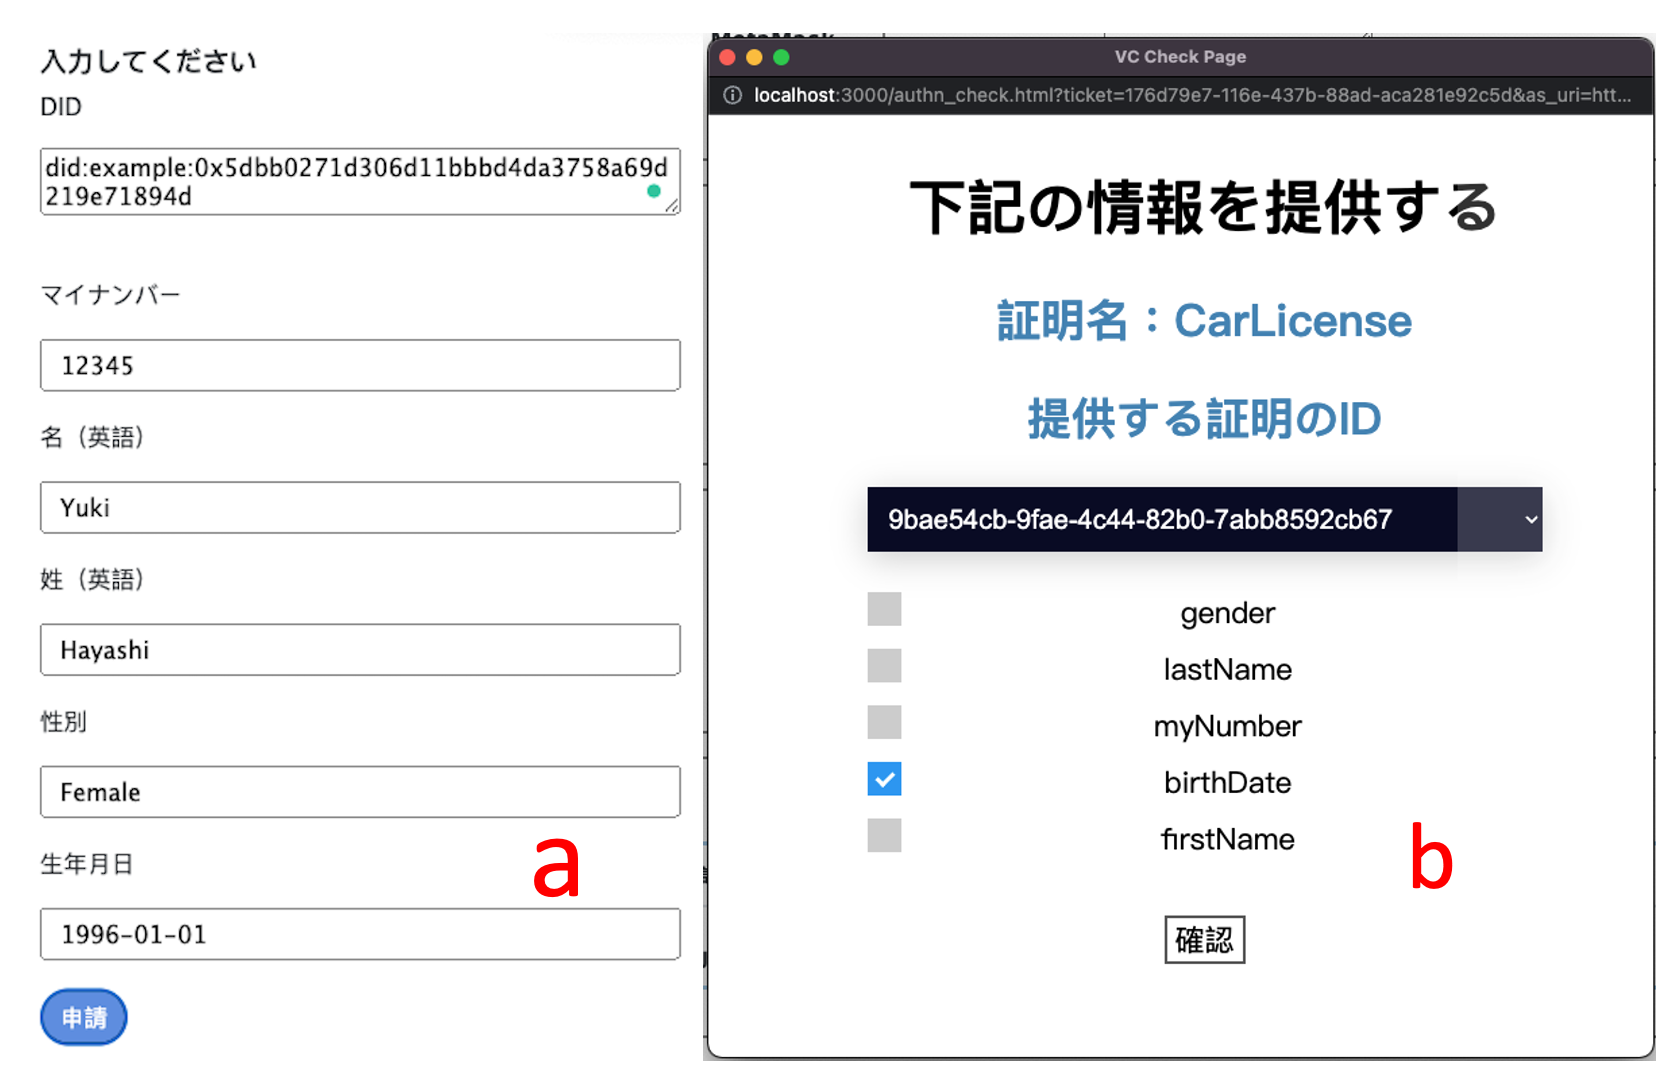
\includegraphics[width=83mm]{images/applyvc_selectclaim.png} %[サイズ]{ファイル名.png}
  \caption{The prototype system. (a) requesting party apply for VC; (b)requesting party select reveal claims in VC} %キャプション
  \label{fig:applyvc_selectclaim} %ラベル名label
  \end{center}
\end{figure}

\begin{figure}[htbp] %浮動式圖形
  \begin{center} %中央寄せ
  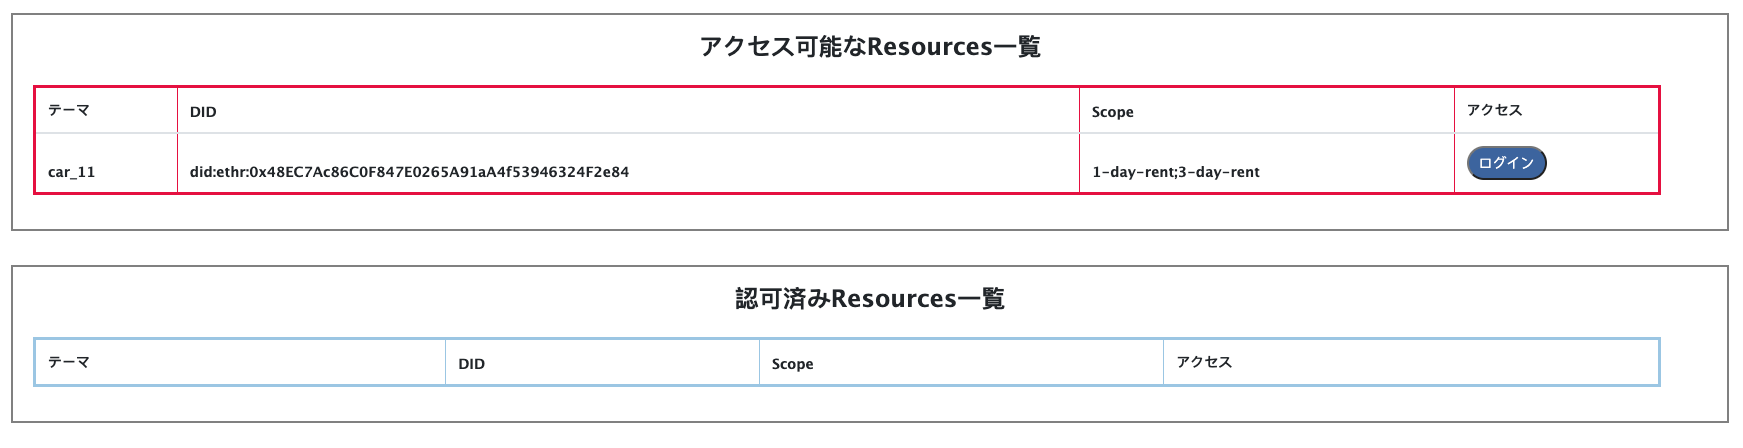
\includegraphics[width=83mm]{images/access_resource.png} %[サイズ]{ファイル名.png}
  \caption{Protected resource web page for the prototype system} %キャプション
  \label{fig:access_resource} %ラベル名label
  \end{center}
\end{figure}

\subsection{Experiments}
To evaluate the feasibility of the authentication flow in the prototype system for a specific implement scenario, the verification time of the VP verification for AS will be an important indicator, which will greatly affect the overall time for the VC-UMA authorization process.
Besides, the data size of VP is also one of the important indicators. If the data size of VP is too large, the authentication process may be not suitable for devices with limited network bandwidth or storage to implement. 
Table \ref{table:experimentsData} shows the result of experiments of the verification time and data size of VP as the number of reveal claims increases (we defined the VP originally including 50 claims).

According to the results, it can be observed that the verification time and data size doesn't significantly increase as the increase of $n$.
This inferred that using the BBS+ Signature to implement the selective disclosure method is a proper way since the cost of time and storage won't increase if we need to reveal more claims in VP.

\begin{table}[htbp]
  \begin{center}
  \caption{Experimental results for Verifiable Presentation Verification Time and Data Size}
  \label{table:experimentsData}
  % \begin{tabular}{c|p{28em}l}
  % \resizebox{\textwidth}{7cm}{
    % \scriptsize 
  \small
  \scalebox{0.9}{
  \begin{tabular}{p{1.4cm} cccccc}
  \hline
  Number of Reveal Claims	& 1 & 10 & 20 & 30 & 40 & 50 \\ \hline\hline
  Verifiable Time (ms)	& 110.4 & 110.8 & 110.6 & 114 & 110.4 & 111.6\\ \hline
  Data Size (byte) 	& 3638 & 3452 & 3268 & 3080 & 2892 & 2708 \\ \hline
  \end{tabular}
  }
  \end{center}
\end{table}

\subsection{Analysis}

Table \ref{table:Evaluation_table} lists the comprehensive comparison between the VC-UMA and other access control mechanisms. \textit{Party-to-Party Authorization} means if the access control mechanism allows resource owner to define party-to-party sharing  scenario;
\textit{Decentralization} illustrates if the common implementation of access control system relies on centralized services for authentication component; \textit{Privacy-preserving Authentication Flow} indicates whether the user can fully control their credential in the access control process or not;
In a nutshell, VC-UMA not only provides an access control mechanism enhancing security and privacy but also provides a more decentralized and more privacy-preserving solution for authentication component in access control compared with other traditional mechanisms. 

% \begin{table}[htbp]
%   \begin{center}
%   \caption{Security and Performance Comparison for Access Control Mechanisms}
%   \label{table:Evaluation_table}
%   % \begin{tabular}{c|p{28em}l}
%   % \resizebox{\textwidth}{!}{
%   \small
%   \scalebox{0.9}{
%     \begin{threeparttable} %添加此处
%       \begin{tabular}{p{1.7cm} >{\centering\arraybackslash}p{1.7cm} ccccc}
%       \hline
%       Mechanism Name/Feature & ID/Password Authentication Access Control & OAuth2 & UMA & VC-UMA \\ \hline\hline
%       Party-to-Party Authorization & - & - & + & + \\ \hline
%       Decentralization & - & - & - & + \\ \hline
%       Privacy-preserving Authentication Flow & - & - & - & + \\ \hline
%       \end{tabular}
%       \begin{tablenotes} %添加此处
%         \item $+$: solved%添加此处
%         \item $-$: unsolved%添加此处
%       \end{tablenotes} %添加此处
%     \end{threeparttable} %添加此处
%   } 
%   \end{center}

% \end{table}

\begin{table}[H]
  \begin{center}
  \caption{Comparison of Access Control Mechanisms in Each Aspect}
  \label{table:Evaluation_table}
  % \begin{tabular}{c|p{28em}l}
  % \resizebox{\textwidth}{!}{

  \begin{threeparttable} %添加此处
    % \begin{tabular}{p{3cm} >{\centering\arraybackslash}p{2cm} ccccc}
    \begin{tabular}{p{1.5cm} >{\centering\arraybackslash}p{0.4cm} >{\centering\arraybackslash}p{0.6cm} >{\centering\arraybackslash}p{0.8cm} >{\centering\arraybackslash}p{0.8cm} >{\centering\arraybackslash}p{0.8cm} >{\centering\arraybackslash}p{0.8cm}}
    \hline
    Mechanism Name/ Feature & UMA & CanDID \cite{CanDID} & Control-Chain \cite{Controlchain}
    & Cred-Chain \cite{Selective_Disclosure_paper} & Lagutin et al. \cite{VC_Oauth} 	& VC-UMA \\ \hline\hline
    Authorization Component & $+$ & $-$ & $+$ & $-$ & $+$ & $+$ \\ \hline
    Authentication Component & $+$ & $+$ & $-$ & $+$ & $+$ & $+$ \\ \hline
    SSI-supported  & $-$ & $+$ &  $-$ & $+$ & $+$ & $+$ \\ \hline
    Party-to-Party Resource Sharing & $+$ &  $-$  & $-$ & $-$ & $-$ & $+$ \\ \hline
    Anonymous Credentials & $-$ & $+$  & $-$ & $+$  & $-$  & $+$ \\ \hline
    \end{tabular}
    \begin{tablenotes} %添加此处
      \item $+$: solved%添加此处
      \item $-$: unsolved%添加此处
      \end{tablenotes} %添加此处
  \end{threeparttable} %添加此处
  % }
  \end{center}

\end{table}

\section{Conclusion}
\label{sec:Conclusion}
This paper proposes a new access control mechanism, VC-UMA, by combining VC technologies with UMA to fill the gap with not defining authentication component in the UMA profile. We demonstrated the VC-UMA mechanism through dynamic and static structures.
By virtue of the decentralized nature of VC, the risks of single node failure and privacy leakage are reduced compared to the common practice which relies on centralized services when implementing UMA.
Besides, since the import of VC needs to be built on a decentralized blockchain infrastructure, this paper is also committed to designing a smart contract API suitable for VC-UMA in order to let authorization server communicate with the blockchain.
On the other hand, considering the privacy issue in VC, this paper also introduces a selective disclosure method so that the requesting party can hide private information when presenting the VC.
Furthermore, to reduce storage consumption and verification time, we choose the BBS+ signature method that has compact features while remaining the high-security level.
Finally, to prove the feasibility of the proposed VC-UMA, the prototype system and the result of the experiments are demonstrated.
As the future work, the complexity of blockchain technology and selective disclosure technologies for VC are expected to be improved to reduce the cost for developers implementing VC-UMA mechanism.



% \section*{References}


\begin{thebibliography}{00}
    \bibitem{AccessControl1}
    P. Samarati and S. C. de Vimercati, ``Access control: Policies, models, and mechanisms,'' {\em in International School on Foundations of Security Analysis and Design}, pp. 137–196, 2000.
  
    \bibitem{UMA}
    E. Maler, M. Machulak, J. Richer, and T. Hardjono, ``User-Managed Access (UMA) 2.0 Grant for OAuth 2.0 Authorization,'' {\em Internet Engineering Task Force}, https://datatracker.ietf.org/doc/draft-maler-oauth-umagrant (accessed Oct. 06, 2021).
  
    \bibitem{UMA_paper1}
    M. P. Machulak, E. L. Maler, D. Catalano, and A. Van Moorsel, ``User-managed access to web resources,'' {\em in Proceedings of the 6th ACM workshop on Digital identity management}, pp. 35–44, 2010.
  
    \bibitem{AccessControl_principle}
    R. S. Sandhu and P. Samarati, ``Access control: principle and practice,'' {\em IEEE Commun. Mag.}, vol. 32, no. 9, pp. 40–48, 1994.
  
    \bibitem{Path_to_Self_Sovereign}
    C. Allen, ``The Path to Self-Sovereign Identity,'' http://www.lifewithalacrity.com/2016/04/the-path-to-self-soverereign-identity.html (accessed Nov. 17, 2021).
  
    \bibitem{VC_model}
    World Wide Web Consortium, ``Verifiable Credentials Data Model v1.1,'' https://www.w3.org/TR/vc-data-model/ (accessed Nov. 22, 2021).
  
    \bibitem{VC_Implementation_Guidelines}
    D. Chadwick, D. Longley, M. Sporny, O. Terbu, and D. Zagidulin, ``Verifiable Credentials Implementation Guidelines 1.0,'' W3C Work. Group Note Sep, 2019.
  
    \bibitem{ssi}
    A. Preukschat and D. Reed, ``Self-sovereign identity,'' {\em Manning Publications}, 2021.
  
    \bibitem{OAuth2}
    D. Hardt et al., ``The OAuth 2.0 authorization framework,'' RFC 6749, October, 2012.
  
    \bibitem{bitcoin}
    S. Nakamoto, ``Bitcoin: A peer-to-peer electronic cash system,'' {\em IEEE Decentralized Bus. Rev.}, p. 21260, 2008.
  
    \bibitem{blockchain_smart_contract}
    X. Xu et al., ``A taxonomy of blockchain-based systems for architecture design,'' {\em in 2017 IEEE international conference on software architecture (ICSA)}, pp. 243–252, 2017.
  
    \bibitem{ethereum}
    V. Buterin, ``A next-generation smart contract and decentralized application platform,'' {\em in White Pap.}, vol. 3, no. 37, 2014.
  
    \bibitem{cl_sig}
    J. Camenisch and A. Lysyanskaya, ``Signature schemes and anonymous credentials from bilinear maps,'' {\em in Annual international cryptology conference}, pp. 56–72, 2004.
  
    \bibitem{bbs_1}
    D. Boneh, X. Boyen, and H. Shacham, ``Short group signatures,'' {\em in Annual international cryptology conference}, pp. 41–55, 2004.
  
    \bibitem{bbs_cl}
    W.Shih, ``Comparing CL Signatures with BBS+ Signatures,'' https://gist.github.com/wayne-shih/46c3d57608d9dcf8e6722d86084e710c (accessed Nov. 18, 2021).
  
    \bibitem{Selective_Disclosure_paper}
    R. Mukta et al., ``Blockchain-based Verifiable Credential Sharing with Selective Disclosure,'' {\em in 2020 IEEE 19th International Conference on Trust, Security and Privacy in Computing and Communications (TrustCom)}, pp. 959–966, 2020.

    \bibitem{Controlchain}
		O. J. A. Pinno, A. R. A. Gregio, and L. C. De Bona,
		\textquotedblleft Controlchain: Blockchain as a central enabler for access control authorizations in the iot\textquotedblright, 
	    in GLOBECOM 2017-2017 IEEE Global Communications Conference, pp. 1–6, 2017.
  
    \bibitem{redactable_signature}
    R. Johnson et al., ``Homomorphic signature schemes,'' {\em in Cryptographers’ track at the RSA conference}, pp. 244–262, 2002.
  
    \bibitem{CanDID}
    D. Maram et al., ``CanDID: Can-do decentralized identity with legacy compatibility, Sybil-resistance, and accountability,'' {\em in 2021 IEEE Symposium on Security and Privacy (SP)}, pp. 1348–1366, 2021.
  
    \bibitem{VC_Oauth}
    D. Lagutin et al., ``Enabling decentralised identifiers and verifiable credentials for constrained IoT devices using OAuth-based delegation,'' {\em in Proceedings of the Workshop on Decentralized IoT Systems and Security (DISS 2019), in Conjunction with the NDSS Symposium, San Diego, CA, USA}, vol. 24, 2019.
  
    \bibitem{geth}
    Ethereum Foundation, ``Go Ethereum,'' https://geth.ethereum.org/ (accessed Nov. 08, 2021).
  
    \bibitem{bbsplus_github}
    MATTR, ``A solution for privacy-preserving verifiable credentials,''  https://github.com/mattrglobal/bbs-signatures (accessed Nov. 16, 2021).
\end{thebibliography}
\vspace{12pt}
\color{red}
IEEE conference templates contain guidance text for composing and formatting conference papers. Please ensure that all template text is removed from your conference paper prior to submission to the conference. Failure to remove the template text from your paper may result in your paper not being published.

\end{sloppypar}
\end{document}
